\begin{figure}[!h]
\centering
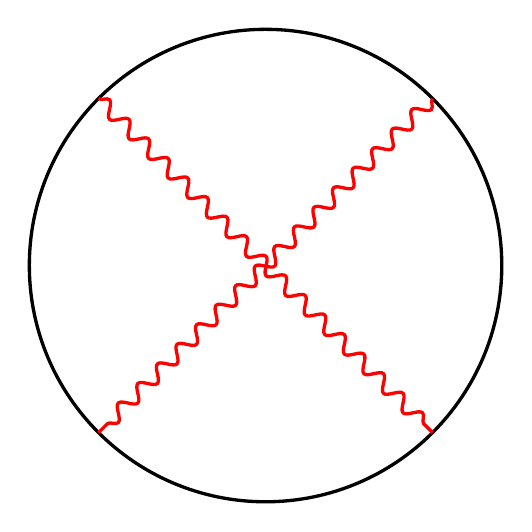
\begin{tikzpicture}[scale=2,>=stealth]
%Draw Circle radius 1 cm
  \def\radi{1.5cm}
    \draw[black,very thick] (0,0) circle (\radi);
   % \foreach \angle/\count in {45/1,135/2,225/3,315/4}
    %    {
        
\tikzset{snake it/.style={decorate, decoration=snake}}
%Draws the 3 acceleration vectors directed inward and offset slightly from the distance vectors
       % \draw [name=acceleration vectors,very thick, snake it]
        %    (\angle:1.2cm) -- node[midway] {} (\angle:0.9cm) ;
         %     \path [draw=blue,snake it](-4,0) -- (-2,0) -- (2,0) -- (4,0);
  %\draw[draw=blue, snake it] (2,0) arc (0:180:2cm);
   % } snake it
    
        \path[coordinate] (0,0)  coordinate(A)++( 45:\radi) coordinate(B1);
        \path[coordinate] (0,0)  coordinate(A)++( 135:\radi) coordinate(B2);
        \path[coordinate] (0,0)  coordinate(A)++( -45:\radi) coordinate(B3);
        \path[coordinate] (0,0)  coordinate(A)++( -135:\radi) coordinate(B4);
        \draw[draw=red, snake it, very thick] (B1)--(B4);
        \draw[draw=red, snake it, very thick] (B2)--(B3);
\end{tikzpicture}
\end{figure}